\section{Aspecto}
\subsection{Temas}

\begin{frame}{Temas}
  \beamer trae por defecto una serie de temas que podemos personalizar. Los temas
  se dividen en 5 tipos:
  \espacio
  \begin{overlayarea}{\textwidth}{.6\textheight}
  \only<1>{
  \begin{block}{Tipos de temas}
    \begin{description}
      \item[Generales]\textbackslash \texttt{\color{keywords}usetheme\{\color{black}nombre\}}
      \item[Internos]
      \textbackslash\texttt{\color{keywords}useinnertheme\{\color{black}nombre\}}
      \\ {\small Entornos de enumeración, bloques...}
      \item[Externos]
      \textbackslash\texttt{\color{keywords}useoutertheme\{\color{black}nombre\}}
      \\ {\small Barras superiores, inferiores y laterales.}
      \item[Colores]
      \textbackslash \texttt{\color{keywords}usecolortheme\{\color{black}nombre\}}
      \item[Fuentes]
      \textbackslash \texttt{\color{keywords}usefonttheme\{\color{black}nombre\}}
    \end{description}
  \end{block}
  }
  \only<2>{
  \begin{exampleblock}{Temas de esta presentación}
    Los temas usados en esta presentación son:
    \espacio
    \ejemplo{temas.tex}
    \espacio
    Para modificar con más detalle utilizamos \texttt{setbeamercolor} y \texttt{setbeamertemplate}.
  \end{exampleblock}
  }
  \end{overlayarea}
\end{frame}

\begin{frame}{Temas}{Temas generales}
  Los temas generales pueden agruparse en varios tipos:
  \espacio
  \begin{itemize}[<alert@+>]
    \item Sin barras de navegación.
    \item Con árbol de navegación.
    \item Con tabla de contenidos lateral.
    \item Con marco de navegación.  \only<4>{Como este!}
    \item Con información sobre sección y subsección.
  \end{itemize}
\end{frame}

\begin{frame}{Temas}
  Los temas disponibles están en la \href{http://www.hartwork.org/beamer-theme-matrix}{\textit{Beamer theme Matrix}}:

  \begin{center}
    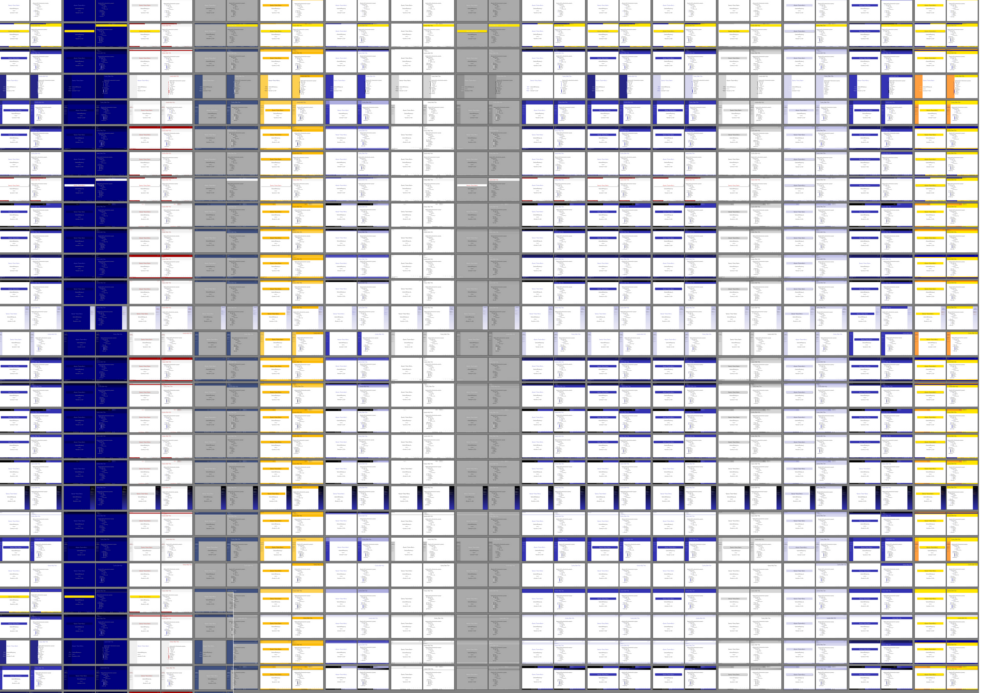
\includegraphics[width=.9\textwidth]{./img/theme-matrix.png}
  \end{center}
  \espacio
\end{frame}

\subsection{Formato}

\begin{frame}{Tamaño y color}
\begin{columns}
  \column{.5\textwidth}
    Cambiamos el tamaño de letra utilizando los comandos habituales en \LaTeX.
    También podemos cambiar el color, utilizando \texttt{xcolor}.

    \espacio

    Los colores básicos son: {\color{white} blanco}, {\color{black} negro},
    {\color{red} rojo}, {\color{green} verde}, {\color{blue} azul},
    {\color{cyan} cian}, {\color{magenta} magenta} y {\color{yellow} amarillo},
    aunque se pueden \href{http://en.wikibooks.org/wiki/LaTeX/Colors}{ampliar y combinar}.
    \espacio

  \column{.5\textwidth}
    \begin{itemize}
      \item \texttt{\tiny \textbackslash tiny}
      \item \texttt{\scriptsize \textbackslash scriptsize}
      \item \texttt{\footnotesize \textbackslash footnotesize}
      \item \texttt{\small \textbackslash small}
      \item \texttt{\normalsize \textbackslash normalsize}
      \item \texttt{\large \textbackslash large}
      \item \texttt{\Large \textbackslash Large}
      \item \texttt{\LARGE \textbackslash LARGE}
      \item \texttt{\huge \textbackslash huge}
    \end{itemize}
\end{columns}
\end{frame}

\begin{frame}{Matemáticas}

Como en cualquier documento de \LaTeX, podemos mostrar expresiones matemáticas
con la sintaxis habitual:
  \begin{equation}
    \mathcal{L} = \frac{-1}{4} F^2  + i\bar{\psi}D\!\!\!\!/\ \psi
  + \bar{\psi}\phi\psi  + h.c.  + |D\phi|^2 - V (\phi)
  \end{equation}

\pause
\begin{alertblock}{Cambiando el tipo de letra}
  \beamer utiliza una letra sin serifa para las fórmulas matemáticas por defecto.
  Podemos utilizar la fuente con serifa
  \href{http://tex.stackexchange.com/questions/34265}{incluyendo}:

  \texttt{{\color{black}\textbackslash}{\color{keywords}usefonttheme}{\color{black} [onlymath]\{serif\}}}
\end{alertblock}
\end{frame}
